\begin{frame}{The geography of the gender gap in 2020}
\label{slide:map}
\begin{figure}[!h]
\centering
\caption{The gender gap in the US in 2020}
\label{fig:gap_map2020}
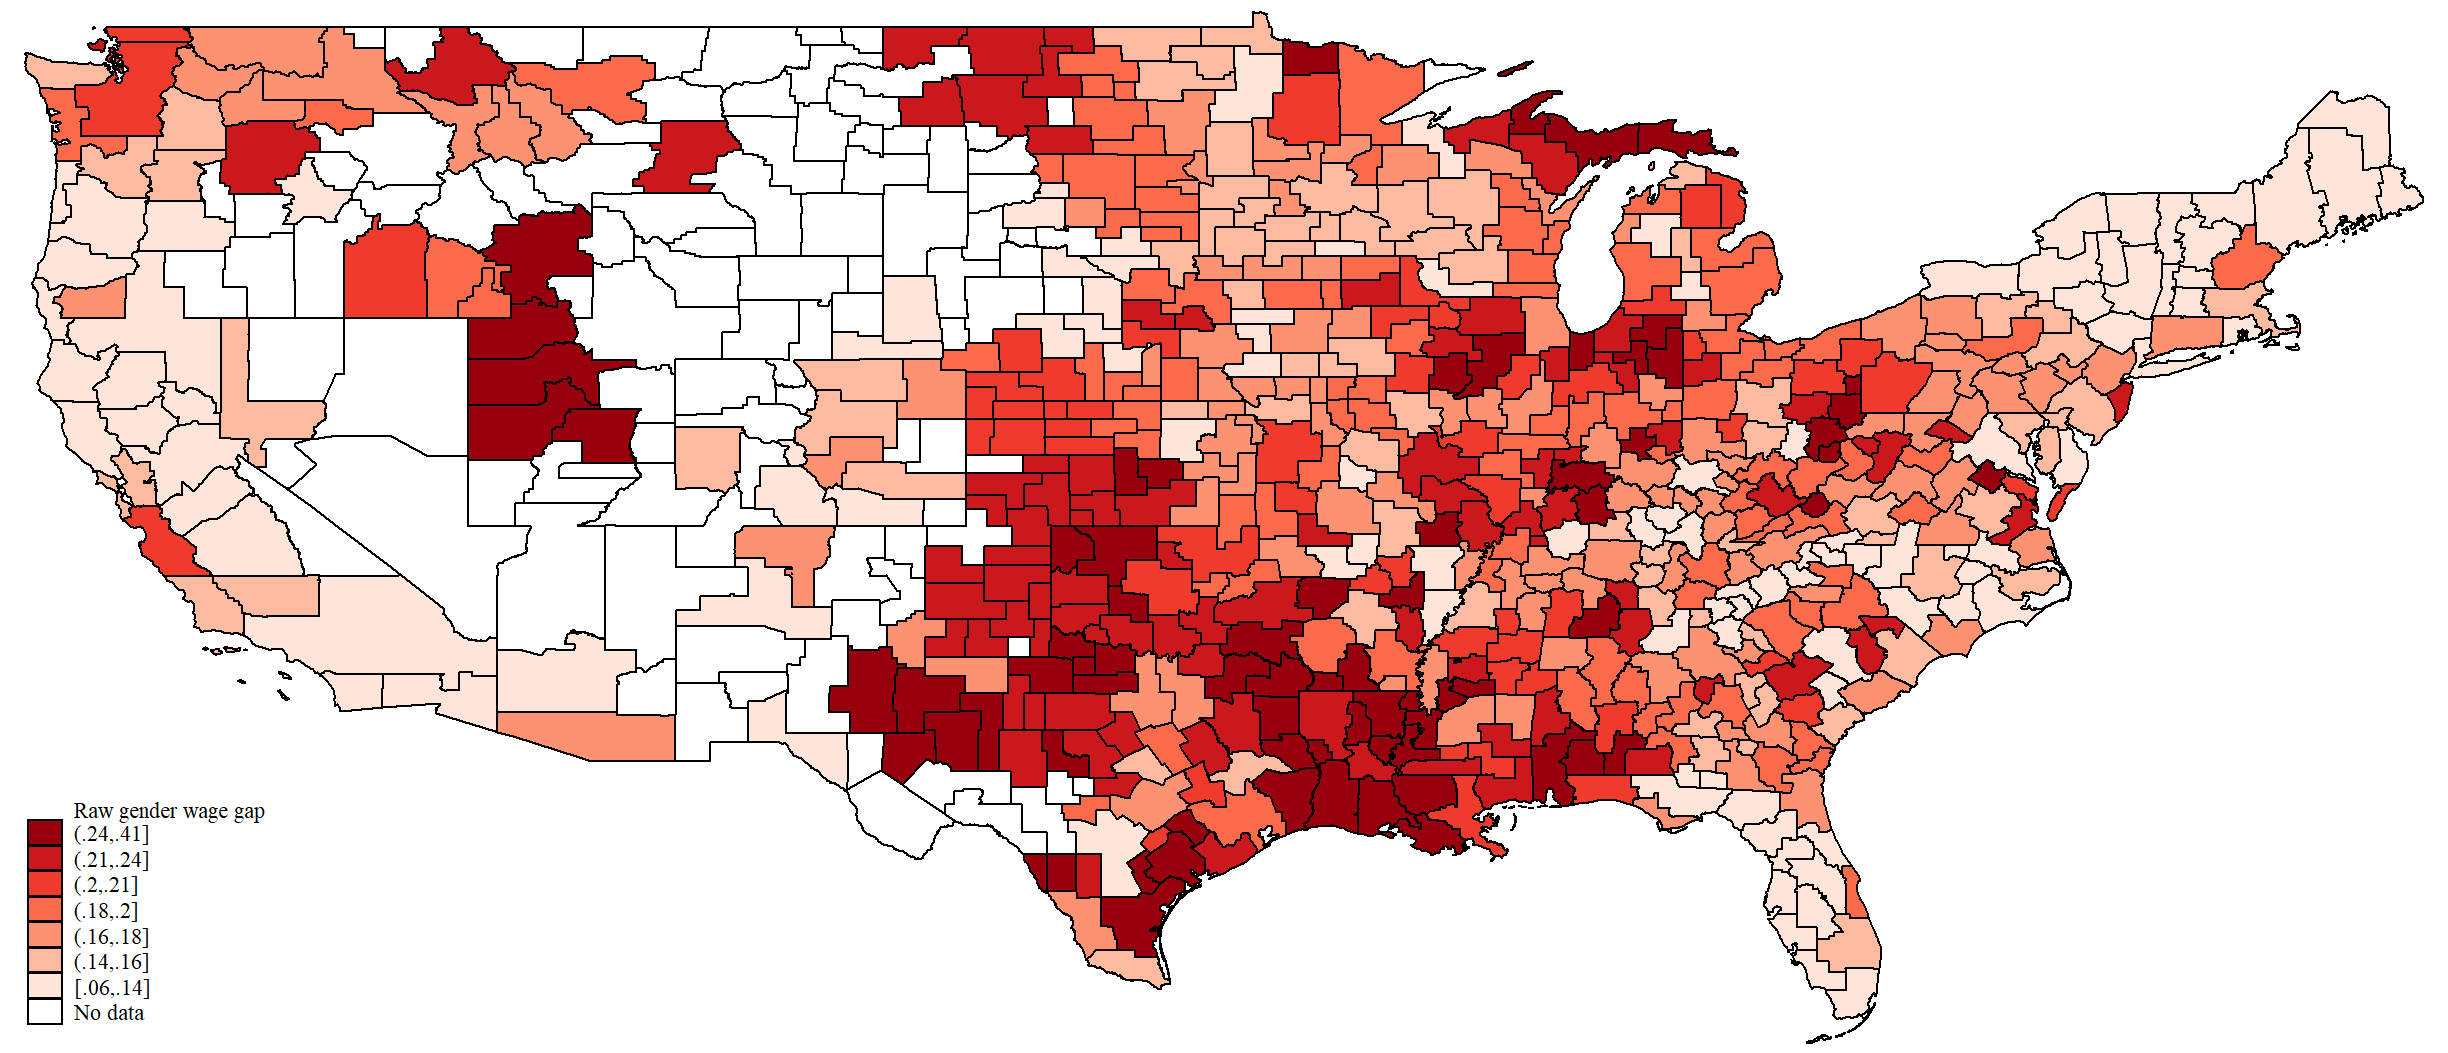
\includegraphics[width=1\textwidth]{../2_analysis/output/figures/raw_wage_map2020_full_time}
\par \begin{minipage}[h]{\textwidth}{\tiny\textbf{Note:} darker colors denote higher relative wages for men. Figure restricts to czones with population densities above 1 person per km$^2$ and full-time year-round workers.}\end{minipage}
\end{figure}

\beamerbutton{\hyperlink{slide:fact1}{Return}}

\end{frame}

\begin{frame}{20-year auto-correlation coefficient is above 50\%} 
	\label{slide:persistence}
	\textbf{\alert{Regression specification:}} $w^{men}_{rt}-w^{women}_{rt}=\alpha_{rt}+\beta_{t}(w^{men}_{rt-j}-w^{women}_{rt-j})$
	\begin{figure}[!h]
\centering
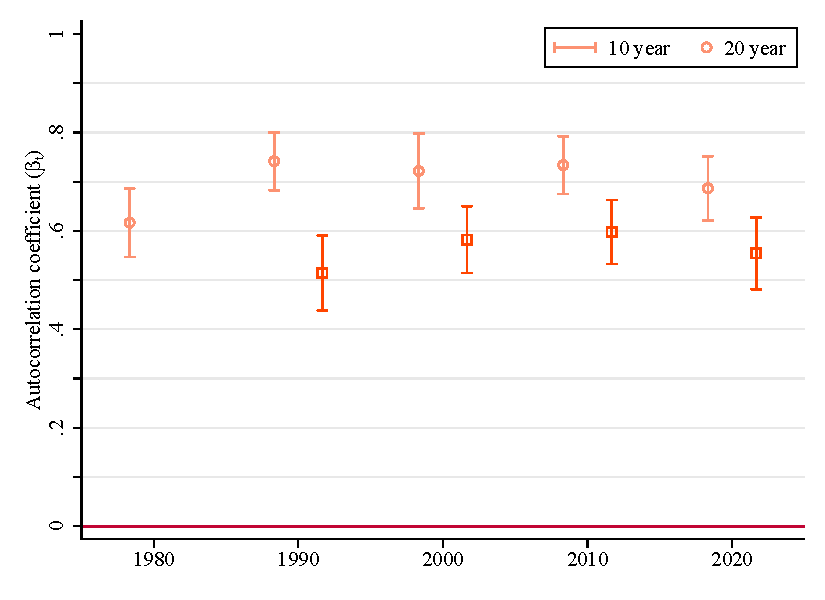
\includegraphics[width=.6\textwidth]{../2_analysis/output/figures/cz_gender_gap_persistence_full_time}
\par \begin{minipage}[h]{\textwidth}{\scriptsize\textbf{Note:} figure restricts to CZ with more than people per km$^2$ and full-time year-round workers.. Bars show 95\% robust confidence intervals. Standard errors are clustered at the CZ level. Dependent and independent variables are standardized}\end{minipage}
\end{figure}

\beamerbutton{\hyperlink{slide:fact1}{Return}}
\end{frame}
\begin{frame}{Residualization procedure}
	\label{slide:residual}
	\begin{enumerate}
		\item Run the regression on \alert{individual} level data:
		\beqns
			wage_{igrt}=X_{igrt}\gamma_t+\lambda_{grt}+\varepsilon_{igrt}
		\eeqns
		where $i,g,r,t$ index individual, sex, CZ and decade respectively. I impose the \alert{same} return on individual level characteristics across sex and CZ.
		\item Run the following regression at the CZ level:
		\beqns
			\lambda_{mrt}-\lambda_{frt}=\alpha_t+\beta_{t}\ln(density)_{rt}
		\eeqns
		no weight is imposed on the CZ-level regressions \citep{Solon2015a}.
		\beamerbutton{\hyperlink{slide:controls}{Return}}
	\end{enumerate}
\end{frame}

\begin{frame}{Low vs high density CZ}
	\label{slide:distribution}
	\begin{figure}[!h]
\centering
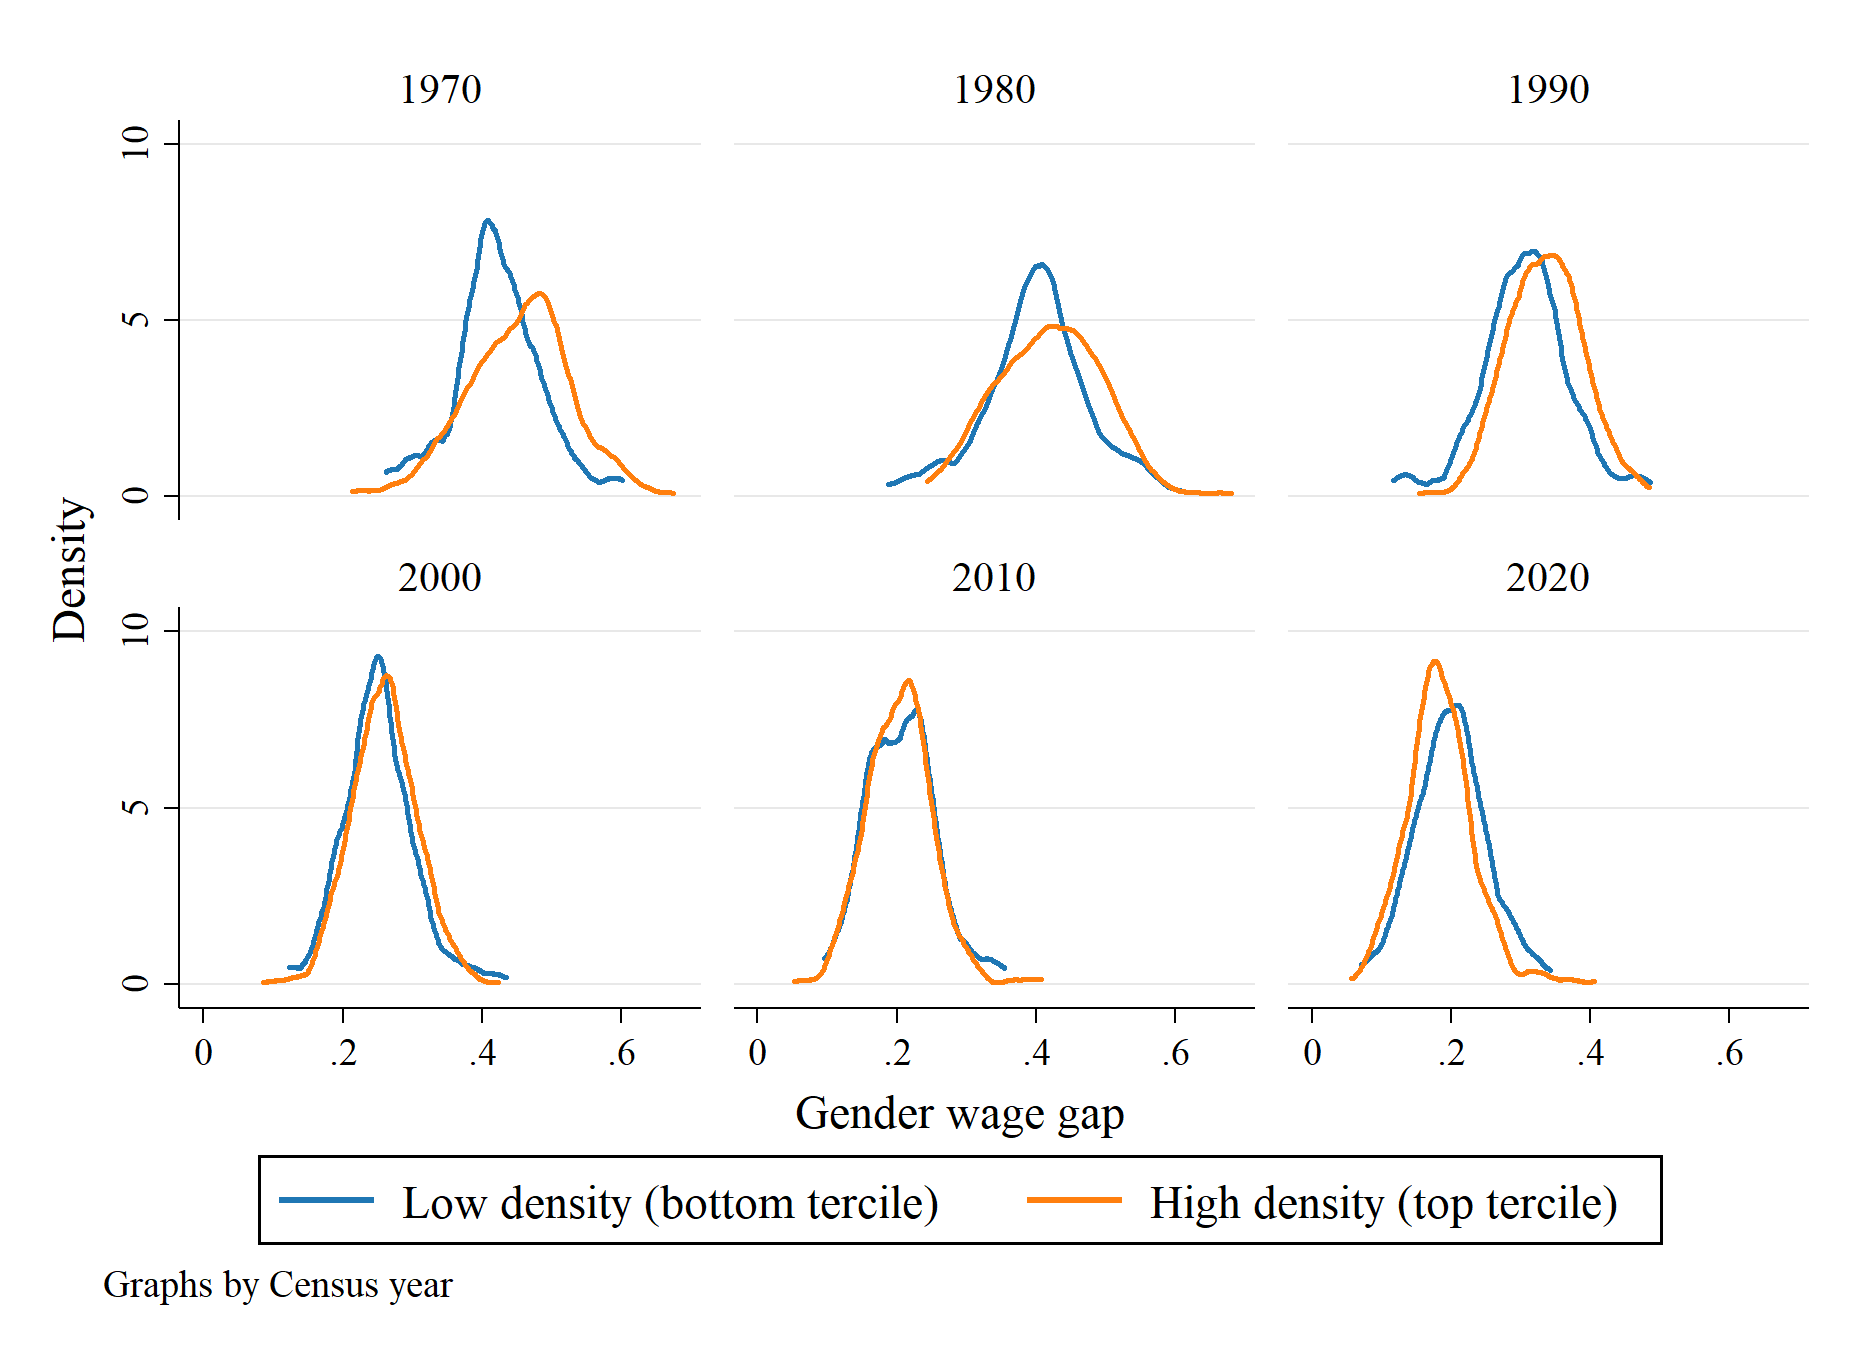
\includegraphics[width=.8\textwidth]{../2_analysis/output/figures/distribution_gap_movement_full_time}
\par \begin{minipage}[h]{\textwidth}{\scriptsize\textbf{Note:} figure restricts to CZ with more than 1 people per km$^2$. Figure generated on 28 Sep 2020 at 15:56:45. Figure generated using the dofile code\_files/kernel\_density\_movement.do.}\end{minipage}
\end{figure}

	\beamerbutton{\hyperlink{slide:baseline}{Return}}
\end{frame}


\begin{frame}{Within-marital status graphs}
	\label{slide:married}
	\textbf{\alert{Regression specification:}}	$w^{men}_{rt}-w^{women}_{rt}=\alpha_{rt}+\beta_{t}\ln(density)_{rt}+ \dots$
	\begin{figure}[!h]
\centering
\caption{Coefficient on population density $ \beta_t $ controlling for worker characteristics}
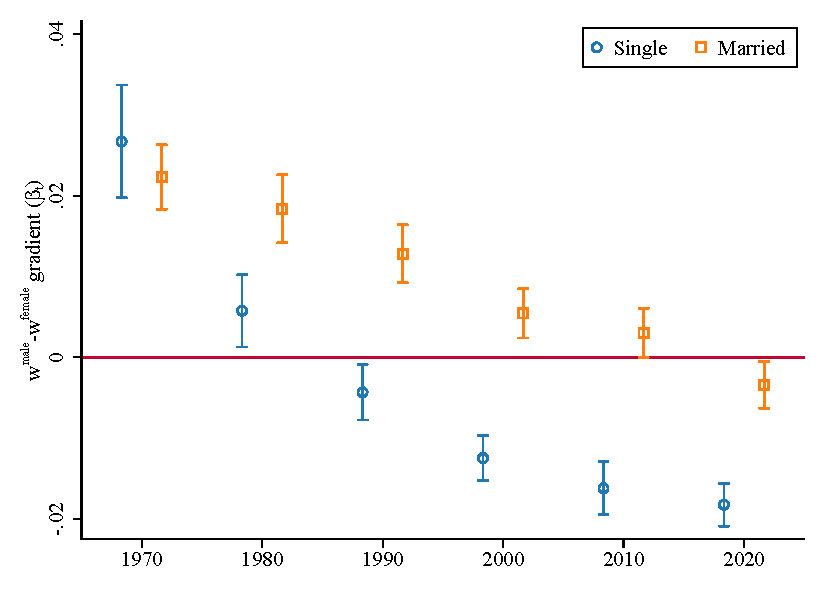
\includegraphics[width=.6\textwidth]{../2_analysis/output/figures/by_married_czone_l_czone_pop_full_time}
\par \begin{minipage}[h]{\textwidth}{\tiny\textbf{Note:} figure restricts to CZ with more than 1 people per km$^2$. Regression includes census division. The regressions are done on data aggregated at the CZ level. Bars show 95\% robust confidence intervals. Standard errors clustered at the CZ level. Figure generated on 20 Oct 2020 at 09:16:34. Figure generated using the dofile 2\_analysis/code\_files/write\_regression\_coefplots.do.}\end{minipage}
\end{figure}

	\beamerbutton{\hyperlink{slide:baseline}{Return}}
\end{frame}

\begin{frame}{Within-having children status graphs}
	\label{slide:has_children}
	\textbf{\alert{Regression specification:}}	$w^{men}_{rt}-w^{women}_{rt}=\alpha_{rt}+\beta_{t}\ln(density)_{rt}+ \dots$
	\begin{figure}[!h]
\centering
\caption{Coefficient on population density $ \beta_t $ conditional conditional on having children}
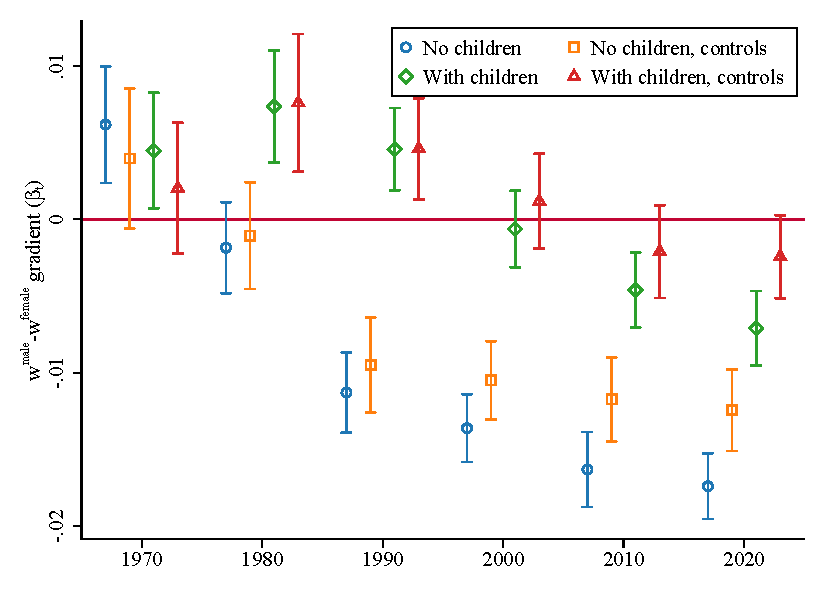
\includegraphics[width=.6\textwidth]{../2_analysis/output/figures/by_children_l_czone_pop_full_time}
\par \begin{minipage}[h]{\textwidth}{\tiny\textbf{Note:} figure restricts to CZ with more than 1 people per km$^2$. Regression includes census division fixed-effects. The regressions are done on data aggregated at the CZ level. Bars show 95\% robust confidence intervals. Standard errors clustered at the CZ level. Figure generated on 20 Oct 2020 at 09:56:35. Figure generated using the dofile 2\_analysis/code\_files/write\_regression\_coefplots.do.}\end{minipage}
\end{figure}

	\beamerbutton{\hyperlink{slide:baseline}{Return}}
\end{frame}


\begin{frame}{Is this about gender? pattern doesn't appear for across race}
	\label{slide:race}
	\textbf{\alert{Regression specification:}}	$w^{white}_{rt}-w^{black}_{rt}=\alpha_{rt}+\beta_{t}\ln(density)_{rt}+ \dots$
	\begin{figure}[!h]
\centering
\caption{Coefficient on population density $ \beta_t $}
\label{fig:race_gradient}
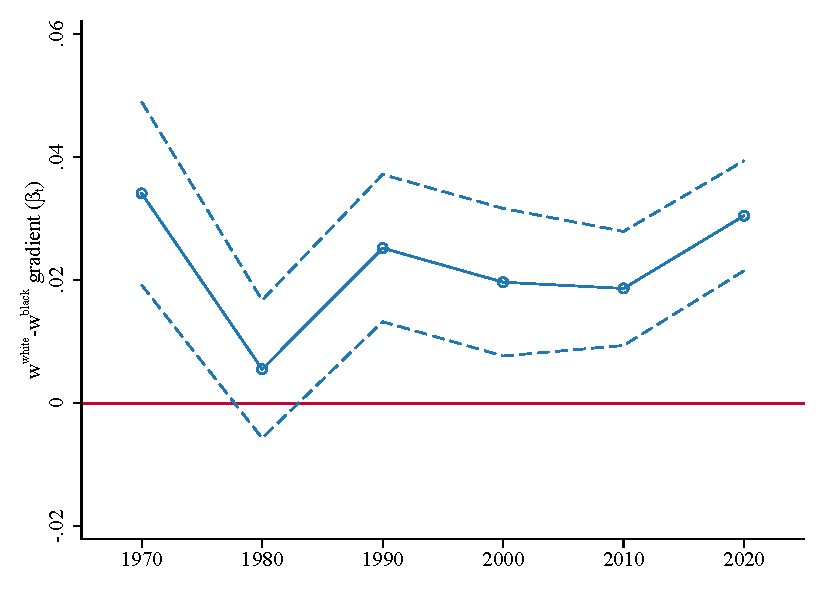
\includegraphics[width=.6\textwidth]{../2_analysis/output/figures/baseline_race_gradients_l_czone_density_full_time}
\par \begin{minipage}[h]{\textwidth}{\tiny\textbf{Note:} figure restricts to CZ with more than 1 people per km$^2$. Bars show 90\% confidence intervals. Standard errors clustered at the CZ level. The figure restricts to year-round full time men workers. Figure generated on 30 Nov 2020 at 11:17:27. Figure generated using the dofile 2\_analysis/code\_files/write\_regression\_coefplots.do.}\end{minipage}
\end{figure}

	\beamerbutton{\hyperlink{slide:baseline}{Return}}		
\end{frame}